\documentclass[12pt]{article} % document type and language

\usepackage{amsmath, amssymb, bm, mathtools, cancel, empheq, ulem, mathrsfs, natbib}
\setcitestyle{aysep={}} 
%\usepackage{newtxmath} 
\usepackage[margin=1in]{geometry}

\usepackage[colorlinks]{hyperref}
\hypersetup{
	colorlinks = true,
	linkcolor=blue,
	citecolor=blue
}

% Allow option to set color when hyperlinking
\newcommand{\MYhref}[3][blue]{\href{#2}{\color{#1}{#3}}}

\date{\today}
\author{Loren Matilsky}
\title{Angular Momentum in Terms of Toroidal and Poloidal Stream Functions}

\input ../macros.tex

\allowdisplaybreaks
\begin{document}
	\maketitle

\section{Prior Work Considered}
In this set of notes, we consider 3D nonlinear dynamo simulations that explored magnetic-field amplitudes at a variety of rotation rates (i.e., enough to make scatter plots of various quantities versus Rossby number and thus theoretically address the activity-rotation relation). We aim to determine what region of parameter space has been explored by global models, and in particular, how the rotation-activity relation may or may not have been addressed. The works considered are:\\

\citet{Christensen2006},\\

\citet{Christensen2009},\\

\citet{Strugarek2017},\\

\citet{Guerrero2019},\\

\citet{Brun2022},\\

\section{Observations of the Stellar Activity-Rotation Relation (ARR)}
The stellar activity-rotation relation (hereafter ARR) has a long history of observation and informs astronomers' generally accepted picture of stellar spin-down. The positive correlation between rotational velocity ($v\sin i$) and chromospheric $\text{Ca}^+$ emission (more or less considered to be linearly proportional to strength of the surface magnetic field) was first noted by \citet{Kraft1967}. This correlation was made famous in the context of spin-down by the ``Skumanich $t^{1/2}$" law. This law states that as a star ages (call its age $t$), its surface magnetic-field strength and rotation rate both decrease like $t^{-1/2}$ \citep{Skumanich1972}. Since spin-down is believed to be caused by angular-momentum loss from a stellar wind, there thus appears to be a negative feedback loop between rotation (which produces magnetic field by a convective dynamo) and magnetic field (which drives the stellar wind and slows the rotation). 

In addition to chromospheric emission, coronal emission (X-ray luminosity) is also found to be proportional to the rotation rate (e.g., \citealt{Walter1982}). Furthermore, the X-ray data show that for a critical rotation rate (corresponding to a critical mixing-length Rossby number of $Ro\sim0.1$), the ratio of X-ray luminosity to total luminosity saturated to a value of $L_X/L_*\sim0.001$. It is still unclear whether this saturation regime corresponds a fundamental dynamo process (for example, the inability of the dynamo to convert additional kinetic energy to magnetic field) or simply geometric effects (for example, the stellar surface becoming so peppered with active regions that it cannot accommodate any more dynamo-produced flux) \citep{Jardine1999}. More recent work \citep{Reiners2022} claims that the saturation regime indicates a fundamental dynamo process.

Since the detailed properties of the magnetic fields in stellar interiors are almost completely unconstrained (including for the Sun), it is reasonable to assume that the overall dynamo strength (defined here to be the rms magnetic-field strength, with the mean taken over the full volume of the star) is proportional to the surface magnetic-field strength, and thus to the proxies of $\text{Ca}^+$ and X-ray flux. With these assumptions, the ARR tells us about two stellar dynamo regimes: slow rotation (where the Sun lies), in which dynamo strength increases with more rapid rotation, and fast rotation, in which the dynamo strength is insensitive to the rotation rate (a saturation regime). Figure \ref{fig:arr} shows the ARR as reported by \citet{Reiners2022}. As the Rossby number $Ro$ (ratio of well-measured rotation period $\prot$ to an ad hoc convective turnover time $\tau$) decreases right to left (i.e., the rotation rate increases), the surface magnetic field strength increases up to a critical Rossby number $Ro=0.13$. After that, faster rotation only leads to marginally increased field strength.

\begin{figure*}\label{fig:arr}
	\centering
	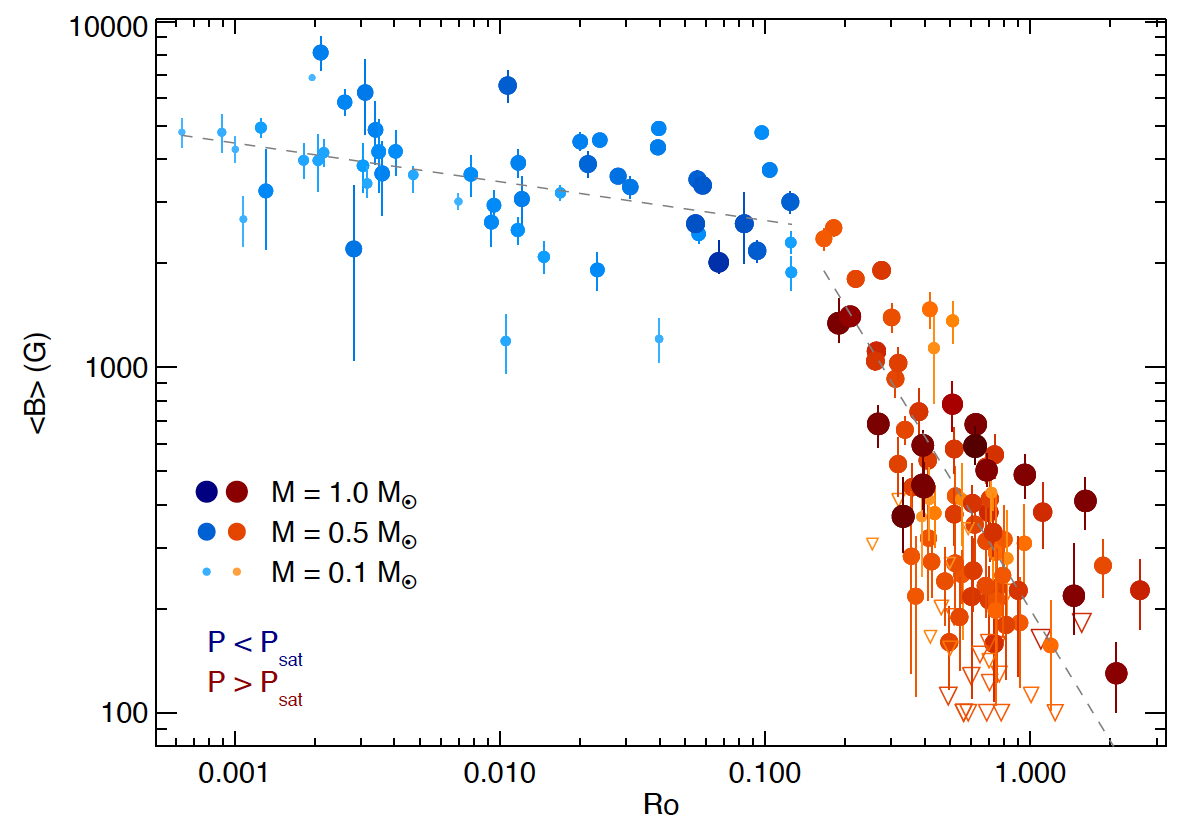
\includegraphics[width=6.5in]{ARR.png}
	\caption{Copied from \citet{Reiners2022}, Figure 5: Magnetic field–rotation relation for solar-like and low-mass stars. Symbols for stars rotating slower than $Ro=0.13$ are colored red, while those of faster rotators are colored blue. Larger and darker symbols indicate higher stellar mass than smaller and lighter symbols.  The gray dashed lines show linear fits separately for the slowly rotating stars ($Ro>0.13$;  $\av{B}=200G\times Ro^{-1.25}$) and the fast rotators ($Ro<0.13$; $\av{B}=2050 G \times Ro^{-0.11}$). Downward open triangles show upper limits for $\av{B}$.}
\end{figure*}

It should be noted that the ``Rossby number" used in plots like Figure \ref{fig:arr} is really an empirical parameter chosen to make the ARR collapse onto a single curve for all different stellar masses (e.g., \citealt{Noyes1984,Pizzolato2003,Wright2011}). In general, the empirical convective turnover time scales like $\tau\sim L_*^{1/2}$, which has some basis in mixing-length theory, but the true dependence of $\tau$ on stellar parameters could be far more complicated. In any case, simply plotting the normalized activity emission (e.g., $L_X/L_*$) with respect to rotation period yields an essentially similar ARR, possibly with different saturation breaks (all in the range of $\prot\sim1$--$3$ days) for different stellar masses (e.g., \citealt{Pizzolato2003}).

\section{Parameters  Spaces Explored}
Global, rotating, magnetized spherical shells are characterized by several non-dimensional parameters. These parameters (which completely characterize the Boussinesq system) are:
\begin{align}
	\text{shell aspect ratio}\quad & \equiv\quad \beta \quad  \equiv\quad  \frac{\rmin}{\rmax},\\
	\text{Rayleigh number} \quad & \equiv \quad {\rm{Ra}} \quad \equiv \frac{g\out\alpha\Delta\tref H^3}{\nu\out\kappa\out},\\
	\text{thermal Prandtl number} \quad & \equiv \quad {\rm{Pr}} \quad = \quad \frac{\nu\out}{\kappa\out},\\
	\text{Ekman number}\quad & \equiv \quad {\rm{Ek}} \quad = \frac{\nu\out}{\Omega_0H^2},\\
	\andd\text{magnetic Prandtl number} \quad & \equiv \quad {\rm{Pr_m}} \quad = \quad \frac{\nu\out}{\eta\out}.
\end{align}
Here, $r$ is the radius, the subscripts ``o" and ``i" refer to the outer and inner radii of the shell (respectively), $H=\rmax-\rmin$ is the shell depth, $g$ is the gravitational acceleration, $\alpha$ is the coefficient of thermal expansion, $\Delta\tref$ is the background (superadiabatic, or adverse) temperature difference between the bottom and top of the shell, $\nu$ is the kinematic viscosity, $\kappa$ the thermal diffusivity, $\Omega_0$ the rotation rate, and $\eta$ the magnetic diffusivity. The ``o" subscripts on the diffusivities and $g$ indicate they are in general functions of $r$. Technically, this radial dependence makes the parameter space accessed by dynamo simulations infinite-dimensional, so hopefully it's not too important! Just kidding.

If the system is anelastic, there are additional parameters because of the stratification. For a polytrope describing a convection zone, these are:
\begin{align}
	\text{shell density contrast}\quad & \equiv \quad {\rm{DC}} \quad \equiv \frac{\rhoref(\rmin)}{\rhoref(\rmax)}\\
	\orr \text{number of density scale heights}\quad &  \equiv \quad N_\rho \quad \equiv \ln{(\rm{DC})}, \\ 
	\text{polytropic index} \quad & \equiv \quad n \quad \equiv \text{something near}\  \frac{3}{2},\\
	\orr 	\text{ratio of specific heats} \quad & \equiv \quad \gamma \quad \equiv \frac{\cp}{\cv}=\frac{n+1}{n}=\text{something near}\  \frac{5}{3},\\
	\andd \text{dissipation number} \quad & \equiv\quad {\rm{Di}}\quad = \quad \frac{g\out H}{\cp \tref\out}.
\end{align}
Here, $\rhoref(r)$ is the background density and $\cp$ is the constant-pressure specific heat. The dissipation number arises because viscous and joule heating are typically neglected in the Boussinesq approximation. 

If there is also a stable layer in the system (say, below the convection zone), some other parameters are needed: the transition location and width, along with the polytropic index of the stable layer or (if the stable layer isn't polytropic) the full entropy gradient $d\sref/dr$ in the stable layer. For polytrope, $n$ determines $d\sref/dr$, which will be a complicated function of $r$ but with an order of magnitude of $[n/(3/2)-1]\cp/\rmin$. Regardless, the stable layer introduces an important, final dimensionless number:
\begin{align}
	\text{buoyancy parameter}\quad & \equiv \quad {\rm{B}} \quad \equiv \frac{\widetilde{N^2}}{\Omega_0^2},\\
	\where N^2 &\equiv \frac{g}{\cp}\frac{d\sref}{dr}
\end{align}
is the squared buoyancy frequency and the tilde indicates a volume average over the stable layer. 

We note also that some authors use a reduced Rayleigh number that is independent of any diffusion coefficient, replacing the diffusion time combination $(H^2/\nu\out)(H^2/\kappa\out)$ with $1/\Omega_0^2$:
\begin{align}
		\text{reduced Rayleigh number} \quad & \equiv \quad {\rm{Ra^*}} \quad \equiv \frac{g\out\alpha\Delta\tref }{\Omega_0^2H}
\end{align}

Finally, in an astrophysical convective system (like a star or the Earth), the adiabatic temperature difference across the convection zone ($\Delta\tref$) is typically unknown. Instead, we can measure the flux driven through the system, and need to define a ``flux-based Rayleigh number" with respect to this flux. For example, we usually know the stellar luminosity $L_*$ and radius $r$. Throughout the star, the different energy fluxes must add up to $\fluxscalar(r)=L_*/4\pi r^2$. If the convection is vigorous, the convective heat transport, or enthalpy flux, should dominate the other fluxes, i.e., $\fluxscalar\sim\rhoref\cp u_rT$, where $u_r$ and $T$ are typical radial velocity and temperature perturbations, respectively. If cold plumes dissipate their energy thermally, we might expect $u_r\sim\kappa\out/H$, or 
\begin{align}
	\text{first flux-based Rayleigh number} \quad & \equiv \quad {\rm{Ra_{F1}}} \quad \equiv \frac{g\out\fluxscalar\out H^4}{\cp\rhoref\out\tref\out\nu\out\kappa\out^2}
\end{align}

Note that the Boulder crew  \citep{Featherstone2016a, Featherstone2016b, Hindman2020, Matilsky2020a, Matilsky2020b, Korre2021, Camisassa2022} use a different "volume-averaged" flux-based Rayleigh number: 
\begin{align}
	\text{second flux-based Rayleigh number} \quad & \equiv \quad {\rm{Ra_{F2}}} \quad \equiv \frac{\tilde{g}\tilde{F}H^4}{\cp\tilde{\rhoref}\tilde{\tref}\tilde{\nu}\tilde{\kappa}^2},
\end{align}
where the tildes refer to volume averages over the convection zone only and $F(r)\equiv\fluxscalar(r)-\fluxscalar_{\rm{rad}}(r)$ is the flux convection and conduction must carry in equilibrium. In the Rayleigh models, $F$ is determined by the volumetric heating $Q(r)$, i.e., $F(r)=(1/r^2)\int_{\rmin}^rQ(x)x^2dx$. 

There is also a reduced flux-based Rayleigh number, used, for example, in \citet{Christensen2006}:
\begin{align}
	\text{reduced flux-based Rayleigh number} \quad & \equiv \quad {\rm{Ra^*_F}} \quad \equiv \frac{1}{4\pi\rmin\rmax} \frac{g\out\alpha Q_{\rm{adv}} }{\rho\out\Omega_0^3H^2}
\end{align}
where $Q_{\rm{adv}}$ is the ``total" (presumably the volume-averaged) integrated convective heat flux. Physically, such a Rayleigh number would be appropriate if the rotation set the typical radial velocity: $u_r\sim H\Omega_0$. 

\section{Christensen \& Aubert (2006)}
\citet{Christensen2006} explored saturated Boussinesq dynamos in the context of planetary magnetic fields 

	%\bibliography{/Users/loren/Desktop/Paper_Library/000_bibtex/library_propstyle,
\bibliography{/Users/loren/Desktop/Paper_Library/000_bibtex/library,
	/Users/loren/Desktop/Paper_Library/000_bibtex/proceedings,
	/Users/loren/Desktop/Paper_Library/000_bibtex/books}
\bibliographystyle{../aasjournal2}

\end{document}